\documentclass[tikz,border=5pt]{standalone}
\usepackage{fontspec}
\setmainfont{Times New Roman}
\usepackage{unicode-math}
\setmathfont{Cambria Math}
\usetikzlibrary{arrows.meta,calc}

\begin{document}
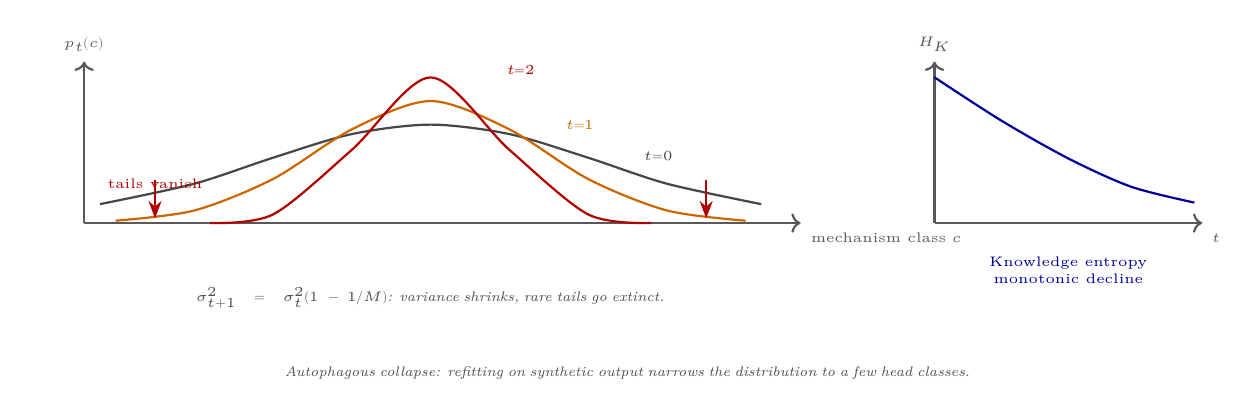
\begin{tikzpicture}[
  arrow/.style={-{Stealth[length=2.2mm]}, thick},
  label/.style={font=\tiny\itshape, text=gray!60!black},
  ax/.style={->, gray!70!black, thick},
]

% === DISTRIBUTION PLOT (left) ===
\draw[ax] (-0.4,0) -- (8.7,0) node[below right,font=\tiny]{mechanism class $c$};
\draw[ax] (-0.4,0) -- (-0.4,2.05) node[above,font=\tiny]{$p_t(c)$};

\draw[thick, gray!55!black] plot[smooth] coordinates {(-0.2,0.24)(1,0.50)(2,0.83)(3,1.13)(4,1.25)(5,1.13)(6,0.83)(7,0.50)(8.2,0.24)};
\draw[thick, orange!80!black] plot[smooth] coordinates {(0,0.03)(1,0.16)(2,0.56)(3,1.19)(4,1.55)(5,1.19)(6,0.56)(7,0.16)(8,0.03)};
\draw[thick, red!70!black] plot[smooth] coordinates {(1.2,0.0)(2,0.11)(3,0.93)(4,1.85)(5,0.93)(6,0.11)(6.8,0.0)};

\node[font=\tiny, text=gray!55!black] at (6.9,0.85) {$t{=}0$};
\node[font=\tiny, text=orange!80!black] at (5.9,1.25) {$t{=}1$};
\node[font=\tiny, text=red!70!black] at (5.15,1.95) {$t{=}2$};

% tail extinction markers
\draw[arrow, red!70!black] (0.5,0.55) -- node[above,font=\tiny,text=red!70!black]{tails vanish} (0.5,0.06);
\draw[arrow, red!70!black] (7.5,0.55) -- (7.5,0.06);

\node[label, align=center, text width=8.5cm] at (4,-0.95)
  {$\sigma_{t+1}^2=\sigma_t^2(1-1/M)$: variance shrinks, rare tails go extinct.};

% === H_K(t) PLOT (right) ===
\begin{scope}[shift={(10.4,0)}]
  \draw[ax] (0,0) -- (3.4,0) node[below right,font=\tiny]{$t$};
  \draw[ax] (0,0) -- (0,2.05) node[above,font=\tiny]{$H_K$};
  \draw[thick, blue!60!black] plot[smooth] coordinates {(0,1.85)(0.85,1.3)(1.7,0.82)(2.5,0.46)(3.3,0.26)};
  \node[font=\tiny, text=blue!60!black, align=center] at (1.7,-0.6) {Knowledge entropy\\monotonic decline};
\end{scope}

\node[label, align=center, text width=15cm] at (6.5,-1.9)
  {Autophagous collapse: refitting on synthetic output narrows the distribution to a few head classes.};
\end{tikzpicture}
\end{document}
